 
\documentclass[./thesis.tex]{subfiles}
 
\begin{document}
\section{Introducion}

La chimie quantique est un domaine qui nécessite d'effectuer des calculs de plus en plus coûteux. En ce qui concerne les méthodes de fonction d'onde, qui sont l'objet de cette thèse, le scaling varie entre $\order{N^5}$ et $\order{N^8}$, avec $N$ le nombre d'électrons du système. Ce scaling très élevé nécessite à la fois la mise en place d'approximations permettant de le réduire, et la conception d'algorithmes efficaces capables de tirer avantage des architectures informatiques modernes. C'est sur ce second aspect que les présents travaux portent plus particulièrement.

La plupart des codes de chimique quantique encore utilisées actuellement (Molpro\cite{Molpro}, Molcas\cite{Molcas}, or Gaussian\cite{g09}\dots), ont débuté leur développement dans les années 90. À cette époque, l'augmentation de la vitesse de calcul était liée à l'augmentation de fréquence des processeurs. Toutefois, depuis une douzaine d'années, celle-ci se heurte à des barrières physiques difficilement franchissables. En conséquence, les accès mémoire, voir disque, ont vu leurs coûts relatifs augmenter,\cite{Wulf1995Mar} et sont devenu le goulot d'étranglement ; de plus, la réduction du temps d’exécution devant dorénavant passer par la multiplication du nombre d'unités de calcul, les algorithmes doivent etre repensés pour des architectures parallèles.\cite{Sutter_2005} De multiples groupes travaillent actuellement à moderniser les codes traditionnels de chimie quantique, jusque-là pensés dans un mode séquentiel. Cette thèse s'inscrit dans cette démarche. 

Certaines méthodes sont de part leur conception même adaptées aux architectures parallèles, en particulier les méthodes de type Monte-Carlo (stochastiques), qui sont par nature composées d'une multitudes de tâches indépendantes, ce qui en rend la parallélisation facile et efficace (\emph{embarassingly parallel}). De plus, elles permettent généralement de déterminer de manière approchée des valeurs dont le calcul exacte est excessivement coûteux. Une partie du travail a consisté à intégrer un aspect Monte-Carlo aux méthodes traditionnelles d'\emph{interaction de configuration} (IC).

Le \QP\cite{QP} développé au LCPQ est une suite de codes de méthodes de fonction d'onde, dont l'objectif premier n'est pas d'être utilisé massivement en production, mais plutôt de permettre le développement et l’expérimentation de nouvelles méthodes de manière simple, y compris pour ce qui est de l'aspect parallèle. Pour cette raison, la base du code est de type \emph{determinant-driven}, c'est à dire itérant sur des déterminants, contrairement à l'approche plus habituelle qui consiste à itérer sur des intégrales biélectroniques (on parle alors d'approche \emph{integral-driven}). Bien que l'approche determinant-driven soit typiquement moins efficace - le nombre de déterminants étant généralement bien supérieur au nombre d'integrales - elle est également moins complexe et plus flexible,\cite{Povill_1995} ce qui rejoint les objectifs du \QP. Si elle s'avère mieux adaptée aux architectures parallèles, elle pourrait connaître un regain de popularité.

La première étape a été l’accélération et la parallélisation de la diagonalisation de Davidson, qui est un point central de toute méthode d'IC. 

Par la suite, il a fallu améliorer l'algorithme de séléction de déterminants utilisé par le \QP pour bâtir des fonctions d'onde compactes. En résumé, cet algorithme de séléction appelé \emph{Configuration Interaction using a Perturbative Selection (CIPSI)},\cite{Huron_1973} consiste à intégrer progressivement à une fonction d'onde variationnelle les déterminants externes avec lesquelles elle interagit le plus.

Les améliorations importantes qui ont été apportées à cet algorithme sont en eux-même le résultat le plus important de ce travail, mais ont également servi de base aux travaux subséquents. En effet, implémenter cette méthode de manière efficace soulève le problème fondamentale de connecter la fonction d'onde à l'espace externe, c'est à dire d’accéder aux informations qu'elle ne contient pas directement. 

La problématique suivante a été de tirer parti au maximum de l'information fournie par l'algorithme CIPSI.

L'une de ces informations est $\EPT$ la contribution perturbative au second ordre, si liée que son calcul est parfois confondu avec l'algorithme CIPSI en tant que sélection. $\EPT$ fournit une approximation de l'énergie de corrélation "perdue" de part la troncature de la fonction d'onde ; de ce fait, si elle est ajoutée à l'énergie variationnelle, elle donne une approximation de l'énergie Full-CI, soit l'énergie exacte du système pour une base donnée. En effet, le critère utilisé par CIPSI pour sélectionner de nouveaux déterminants, est leurs contribution perturbative au second ordre, calculée pour chaque déterminant externe (approximations mises à part) ; la somme de ces contributions n'est nul autre que $\EPT$, qui peut donc, en principe, être calculée au cours de l'algorithme de sélection. Toutefois, en pratique, la sélection peut subir des approximations bien plus drastiques que le calcul de $\EPT$, car identifier les contributions les plus importantes peut se passer d'explorer des espaces de déterminants externes dans lesquelles les contributions seront prévisiblement petites, ou même de calculer les contributions avec précision. Calculer la somme des contributions, en revanche, peut difficilement se passer d'être précis et exhaustif, de part l'effet de masse.

Pour cette raison, le calcul de $\EPT$ - tel qu'implémenté, comme un ``sous-produit'' de la sélection - était bien plus coûteux que la sélection, et souvent trop coûteux, ce qui conduisait en pratique à tronquer le calcul. Ce problème à pu être réglé par l'intégration d'un aspect Monte-Carlo, afin d'en retirer les bénéfices habituels, à savoir un résultat d'une précision acceptable pour une fraction du coût, et une parallélisation relativement simple et efficace.

Nous avons ensuite pu déplorer que notre calcul de $\EPT$, alors qu'il fournit des informations détaillées sur les interactions entre la fonction d'onde et l'espace externe, ne permette qu'une correction globale de l'énergie, et pas de la fonction d'onde elle-même. En se basant sur la méthode dite shifted-\Bk et l'utilisation de matrices habillées,\cite{Nitzsche_1978a, Nitzsche_1978b, Rawlings_1983, Kozlowski_1995, Kozlowski_1994a, Kozlowski_1994b, Kozlowski_1994c} la fonction d'onde a pu être corrigée en fonction des informations obtenues lors du calcul de $\EPT$ ; puis de manière plus générale, un système permettant de raffiner la fonction d'onde sous l'effet d'un espace externe estimé stochastiquement a été mis en place. Ce système a été testé avec l'espace externe impliqué par l'approche shifted-\Bk (où les coefficients des déterminants externes sont estimés perturbativement) et par une approche de type MR-CCSD développée précédemment.

Les considérations techniques de ces implémentations n'ont bien sûr pas été abordées en détails dans les différents articles produits au cours de cette thèse. En ce qui me concerne, mon travail a porté sur les implémentations au moins autant que sur la théorie sous-jacente, c'est pourquoi ce manuscrit est une opportunité d'aborder les questions algorithmiques plus en détail. Dans la mesure où ces questions pourraient être d'un interet particulier pour ceux cherchant à comprendre en profondeur l'implémentation du \QP, j'ai choisi de le rédiger en anglais.

\section{Calcul \emph{determinant-driven} des éléments de matrice de $\widehat H$}

Un déterminant de Slater (simplement appelé ``déterminant'' dans la suite du texte) peut être vu comme un ensemble d'opérateurs de création agissant sur le vide.


\begin{equation}
\ac{i} \ac{j} \ac{k} \vac = \ket{I}
\end{equation}

De part la nature fermionique des électrons, permuter deux opérateurs conduit à un changement de signe.

\begin{align}
\ac{j} \ac{i} & = -\ac{i} \ac{j} \\
\ac{j} \ac{i} \ac{k} \vac &=  -\ket{I}
\end{align}

On peut voir qu'un déterminant peut se décomposer en deux informations :

\begin{itemize}
\item
L'ensemble des spinorbitales occupées.
\item
Un signe, ou ``facteur de phase''.
\end{itemize}
L'approche determinant-driven implique d'itérer sur des déterminants, et par conséquent, nécessite de calculer explicitement et de manière intensive des éléments de matrice de $\widehat H$ l'hamiltonien électronique non-relativiste.
C'est ce que permettent les règles de Slater-Condon. Avec $\ket D$ un déterminant de Slater et $\ket {D_{pq}^{rs}}$ le déterminant obtenu à partir de $\ket D$ par la substitution des spinorbitales $p$ et $q$ par les spinoribtales $r$ et $s$ ; en d'autres termes par l'action de l'opérateur d'excitation $\hat T_{pq}^{rs}$ :
\begin{align}
\Hij{D}{D} & = \sum_{i\in \ket{D}} \mel{i}{\hat{h}}{i} + \frac{1}{2} \sum_{i\in \ket{D}} \sum_{j\in \ket{D}} \Big [ (ii|jj) - (ij|ij) \Big ]      \\
\Hij{D}{D_p^r} & = \mel{p}{\hat{h}}{r} + \sum_{i\in \ket{D}} \Big [ (pr|ii) - (pi|ri) \Big ]        \\
\Hij{D}{D_{pq}^{rs}} & = (pr|qs) - (ps|qr) \\
\Hij{D}{D_{pqt \ldots}^{rsu \dots}} & = 0
\end{align}
avec $\hat{h}$ la partie mono-électronique (énergie cinétique et potentiel électron-noyau),
\begin{equation}
\mel{p}{\hat{h}}{r} = \int d{\bf x}\; \phi^*_p(\mathbf{x}) \qty( -\frac{1}{2}\nabla + V_1(\mathbf{x})) \phi_h(\mathbf{x}),
\end{equation}
$i \in \ket{D}$ signifiant que la spinorbitale $i$ est occupée dans le déterminant $\ket{D}$, et
\begin{equation}
(ij|kl) = \int d{\bf x}_1 \int d{\bf x}_2 \; \phi^*_i({\bf x}_1)\phi_j({\bf x}_1) \frac{1}{|{\bf r}_1 - {\bf r}_2|} \phi^*_k({\bf x}_2)\phi_l({\bf x}_2)
\end{equation}
une intégrale biélectronique.
Ainsi qu'on le voit, ces calculs impliquent :
\begin{itemize}
\item
D'être capable de déterminer l'excitation liant deux déterminants.
\item
De pouvoir accéder rapidement aux intégrales biélectroniques correspondantes.
\end{itemize}

Les intégrales biélectroniques étant potentiellement trop nombreuses pour être directement indicées à partir des indices d'orbitale qui la définissent - cela nécessiterait un stockage de l'ordre de $\Norb^4$ avec $\Norb$ le nombre d'orbitales - une table de hash est un choix naturel pour stocker et accéder aux éléments non-nuls en temps constant. Une table de hash ``maison'' spécifiquement conçue pour les intégrales est implémentée dans le \QP. Dans le cas où les intégrales recherchées sont aléatoires, elle permet un accès seulement deux fois plus lent qu'un accès direct dans un tableau à 4 dimensions. Cette différence s'accentue toutefois dans le cas où l'accès suit un certain schéma ; en pratique, un calcul CIPSI complet est de l'ordre de deux fois plus long si il utilise une table de hash plutôt qu'un accès direct. Pour atténuer ce problème, les intégrales impliquant uniquement les 128 orbitales les plus proches du niveau de Fermi sont stockées dans un tableau à 4 indices (2 Gio).

Les déterminants sont stockés avec la représentation dite \emph{bitstring}. Cette approche est fondamentale dans l'implémentation du \QP. Chaque spinorbitale est associée à un bit (contenu dans une variable de type integer 64 bits), qui prend la valeur de son nombre d'occupation. En d'autres termes $0$ est associé au statut "inoccupé" et $1$ au statut "occupé". Une variable integer de 64 bits peut donc stocker l'occupation de 64 spinorbitales. Le nombre de variables integer nécessaire pour stocker $\Norb$ spinorbitales est
\begin{equation}
\Nint = \left \lfloor \frac{\Norb-1}{64} \right \rfloor + 1.
\end{equation}

Pour des raisons pratiques, les spinorbitales $\uparrow$ et $\downarrow$ sont stockées sur des variables séparées. Par conséquent, la représentation interne d'un déterminant est un tableau à 2 dimensions, la dimension externe de taille $2$ (spin $\uparrow$ et $\downarrow$), et l'interne de taille $\Nint$.

Cette représentation ne permet toutefois pas de stocker le facteur de phase, par conséquent cette elle ne peut stocker qu'une ``valeur absolue'' de déterminant.

La représentation bitstring est une manière compacte de stocker des déterminants, mais c'est plus qu'une méthode de stockage ; en effet, elle permet de tirer parti de la capacité des processeurs à effectuer des opérations bit à bit de manière efficace. Plutôt que d'interpréter cette représentation comme une liste de nombres d'occupations, on peut l'interpréter comme la définition d'un ensemble.

On appel bitstring un tableau d'integers 64 bits de taille $\Nint$, et d'une manière générale, il peut définir un ensemble d'orbitales ; les orbitales contenues dans l'ensemble sont celles dont le bit associé est non nul. La représentation d'un déterminant peut alors être vue comme une paire de bitstrings associés aux spinorbitales $\uparrow$ et $\downarrow$, respectivement, et donc définissant un ensemble de spinorbitales (en l’occurrence, les spinorbitales occupées). On appel de tels objet des $\uparrow\downarrow$-bitstrings.
\lstset{frame=single}
\begin{lstlisting}
  ! I est un updown-bitstring
  ! I_up et I_down sont des bitstrings
  
  integer*8 :: I(N_int, 2)
  integer*8 :: I_up(N_int), I_down(N_int)
  ...! On charge un determinant dans I
  I_up   (:) = I(:,1)
  I_down (:) = I(:,2)
\end{lstlisting}
\lstset{frame=none}

Certaines instructions disponibles sur les processeurs modernes peuvent être ramenées à des opérations sur des ensembles. L'instruction AND par exemple (\emph{bitwise AND}, fonction $\text{\texttt{IAND}}$ en Fortran), correspond à l'intersection.

\begin{equation}
A = \IAND{B}{C}
\end{equation}
Si on interpréte $A$, $B$ et $C$ comme des bitstrings, $A$ définit l'intersection entre $B$ et $C$.
A titre d'exemple, en utilisant les instructions suivantes:
\begin{sloppypar}
\begin{itemize} 
        \item $\POPCNT{\bitI}$ :
        Retourne le nombre de bits non nuls dans un integer $\bitI$. \\
        ${\POPCNT{\binary{00011000}} = 2}$.
         
        \item $\IEOR{\bitI}{\bitJ}$ : ``ou exclusif'' bit à bit. \\
        ${\IEOR{\binary{1100}}{\binary{1010}} = \binary{0110}}$.
              
              
        \item $\IAND{\bitI}{\bitJ}$ : ``et'' bit à bit. \\
        ${\IAND{\binary{1100}}{\binary{1010}} = \binary{1000}}$.
\end{itemize}
\end{sloppypar}
On peut déterminer le degré ainsi que les les trous et particules impliqués dans une excitation.
Avec $B$ et $C$ les $\uparrow \downarrow$-bitstrings définissants deux déterminants $\ket B$ et $\ket C$ (par soucis de simplification on oublie leur caractère de tableau) :
\begin{equation}
d = \POPCNT{\IEOR{B}{C}}
\end{equation}
En toutes lettres, $d$ est le nombre de spinorbitales qui sont occupées dans exactement l'un de $\ket B$ ou de $\ket C$, autrement dit celles dont l'occupation diffère  ; une excitation impliquant un changement d'occupation dans 2 spinorbitales, le degré d'excitation entre $\ket B$ et $\ket C$ est de $d/2$.

Ensuite :
\begin{equation}
A = \IAND{C} {\IEOR{B}{C}}
\end{equation}

Ici $A$ est un $\uparrow \downarrow$-bitstring qui, en toutes lettres, contient les spinorbitales présentes dans $\ket C$ et dont l'occupation diffère entre $\ket B$ et $\ket C$. Autrement dit, les particules impliquées dans l'excitation $\hat T$ telle que $\ket C = \hat T \ket B$. De la même manière les trous impliqués dans $\hat T$ sont déterminés par $\IAND{B} {\IEOR{B}{C}}$

Puisque notre représentation en $\uparrow \downarrow$-bitstring ne stock pas le signe d'un déterminant, lorsqu'une excitation est appliquée, il faut calculer un facteur de phase, qui peut être de $1$ ou $-1$. Pour une excitation $\hat T_p^q$, ce facteur est lié à la parité du nombre d'électrons entre les spinorbitales $p$ et $q$. Dans la mesure où le facteur de phase doit être calculé de nombreuses fois sur un même déterminant, une manière efficace de le faire consiste à stocker pour chaque spinorbitale, le nombre d'électrons dans les spinorbitales inférieures ; il suffit ensuite d'une soustraction pour connaître le nombre d'électrons entre deux spinorbitales. En pratique, il n'est pas nécessaire de stocker le nombre, mais seulement sa parité (connaissant les parités de $A$ et $B$ il est trivial de déterminer la parité de $A-B$) ; ce type de stockage est appelé \emph{phase mask}.
\section{Diagonalisation de Davidson}

D'un point de vu algorithmique, la question posée se résume au calcul (mais pas au stockage) de la matrice hamiltonienne. Le calcul d'un élément de matrice peut être fait efficacement, mais le calcul de chacun des $\Ndet^2$ éléments (avec $\Ndet$ le nombre de déterminants dans la fonction d'onde variationnelle) reste extrêmement coûteux.

Afin de réduire le nombre d'éléments à considérer, on peut créer des sous-ensembles de déterminants identifiables comme entièrement déconnectés de certains autres sous-ensembles. Ainsi, les déterminants peuvent par exemple être regroupés en fonction de leur partie de spin $\uparrow$. Si la partie $\uparrow$ qui définie un groupe, est plus que doublement excitée par rapport à la partie $\uparrow$ qui définie un autre groupe, on peut immédiatement en déduire qu'aucune connexion ne pourra être trouvée entre les déterminants de l'un et de l'autre groupe.

La version implémentée, pour une meilleur efficacité, disjoint les différents types d'excitation.
\begin{itemize}
\item
Excitations $\uparrow \uparrow$ et $\uparrow$: les déterminants liés par une telle excitation partagent par définition la même partie de spin $\downarrow$. Les déterminants sont donc regroupés en fonction leur partie de spin $\downarrow$, et chaque déterminant n'a besoin d'être comparé qu'aux déterminants du même groupe. Du fait le la faible taille des groupes, cette recherche est très peu coûteuse.
\item
Excitations $\downarrow \downarrow$ et $\downarrow$ : situation symétrique avec la précedente, les déterminants sont donc groupés en fonction de leur partie de spin $\uparrow$.
\item
Excitations $\uparrow \downarrow$ : la vaste majorité du temps de calcul est consacré à celles-ci. Les déterminants sont regroupés selon leur partie $\uparrow$ (arbitrairement). Une excitation $\uparrow \downarrow$ ne pourra être trouvée qu'entre deux groupes dont les parties $\uparrow$ qui les définissent sont simplement excitées l'une par rapport à l'autre.
\end{itemize}
\section{Sélection avec le critère CIPSI}

L'algorithme CIPSI consiste à construire itérativement la fonction d'onde variationnelle, en lui ajoutant à chaque itération les déterminants externes qui interagissent le plus avec elle.

L'itération $n$ du CIPSI peut être décrite comme suit:
\begin{enumerate}
\item
La fonction variationnelle $\ket {\Psi^{(n)}}$ est définie sur un ensemble de déterminants $\{\ket{D_I}\}^{(n)}$ dans lequel on diagonalise $\widehat{H}$
\begin{equation}
\ket{\Psi^{(n)}} = \sum_{I} c_I^{(n)} \kI
\end{equation}
%The determinants in $\{\ket{D_I}\}^{(n)}$ will be characterized as \emph{internal}.
\item

Pour chaque déterminant $\kalpha$ dit \emph{externe}, $\kalpha \notin \{\ket{D_I}\}^{(n)}$, on calcul la contribution perturbative

\begin{equation}
e_\alpha = \frac{\Hij{\Psi^{(n)}}{\alpha}^2}{E^{(n)} - \Hij{\alpha}{\alpha}}.
\end{equation}
$E^{(n)}$ dépend de la théorie de perturbation utilisée (dans notre cas, Epstein-Nesbet, $E^{(n)}$ correspond à l'énergie variationnelle de $\ket{\Psi^{(n)}}$. Toutefois une autre théorie pourrait être utilisée).
%As we use Epstein-Nesbet perturbation theory, $E^{(n)}=\Evar^{(n)}$ is the variational energy of the wave function at the current iteration (note that another perturbation theory could be used here).
\item
On extrait $\{ \ket{\alpha_\star} \}^{(n)}$ le sous-ensemble des déterminants $\kalpha$ de plus grande contribution $e_\alpha$, et on les ajoute à la fonction variationnelle.
\begin{equation}
\{\ket{D_I}\}^{(n+1)} = \{\ket{D_I}\}^{(n)} \cup \{ \ket {\alpha_\star} \}^{(n)}
\end{equation}
\item
On passe à l'itération $n+1$ si un critère d’arrêt n'est pas atteint.
\end{enumerate}
L'ancienne implémentation réalisait cet algorithme de manière relativement naïve, chaque déterminant externe étant généré individuellement puis comparé à chaque déterminant de la fonction d'onde variationnelle.
Le très important gain de performance repose sur deux améliorations:
\begin{itemize}
\item
Le filtrage des déterminants internes. Les déterminants externes sont créés en prenant un déterminant interne, qualifié de \emph{générateur}, et en lui appliquant toutes des simples et doubles excitations possibles, en d'autres termes en créant tous les déterminants qui lui sont connectés. Chacun des déterminant externe ainsi généré, doit être comparé à chaque déterminant interne pour le calcul de $e_\alpha$. Ainsi, pour qu'un déterminant interne soit connecté à un déterminant externe, il ne peut pas être ``éloigné'' du générateur par plus de 4 excitations. Par conséquent, tous les déterminants plus que quadruplement excités par rapport au générateur courant, peuvent être ignorés dans le calcul des $e_\alpha$. Ce filtrage peut être raffiné quand le générateur devient un générateur doublement ionisé, ainsi que sera discuté dans le point suivant.
\item
La détermination ``par batch'' des connexions. 
Plutôt que de considérer les déterminants externes ``un par un'', l'unité de base est un générateur doublement ionisé $\ket {G_{pq}}$, soit $\ket G$ ionisé dans les spinorbitales $p$ et $q$. Il implique les déterminants $\hat T_{pq}^{rs} \ket G$ pour toutes les valeurs de $r$ et $s$ ; en effet, comparer $\ket {G_{pq}}$ à un déterminant interne, permet de déterminer systématiquement quelles sont les valeurs de $r$ et $s$ qui correspondent à un déterminant connecté au dit déterminant interne.
De même qu'on a pu filtrer certains déterminants internes en fonction du générateur, on peut en filtrer en fonction des ionisations $p$ puis $q$.
\end{itemize}
On peut tenter de résumer la différence entre l'ancienne et la nouvelle implémentation à l'aide des figures \ref{fig:old_cipsi_fr} et \ref{fig:new_cipsi_fr}.
\begin{figure}[h!]
        \begin{center}
                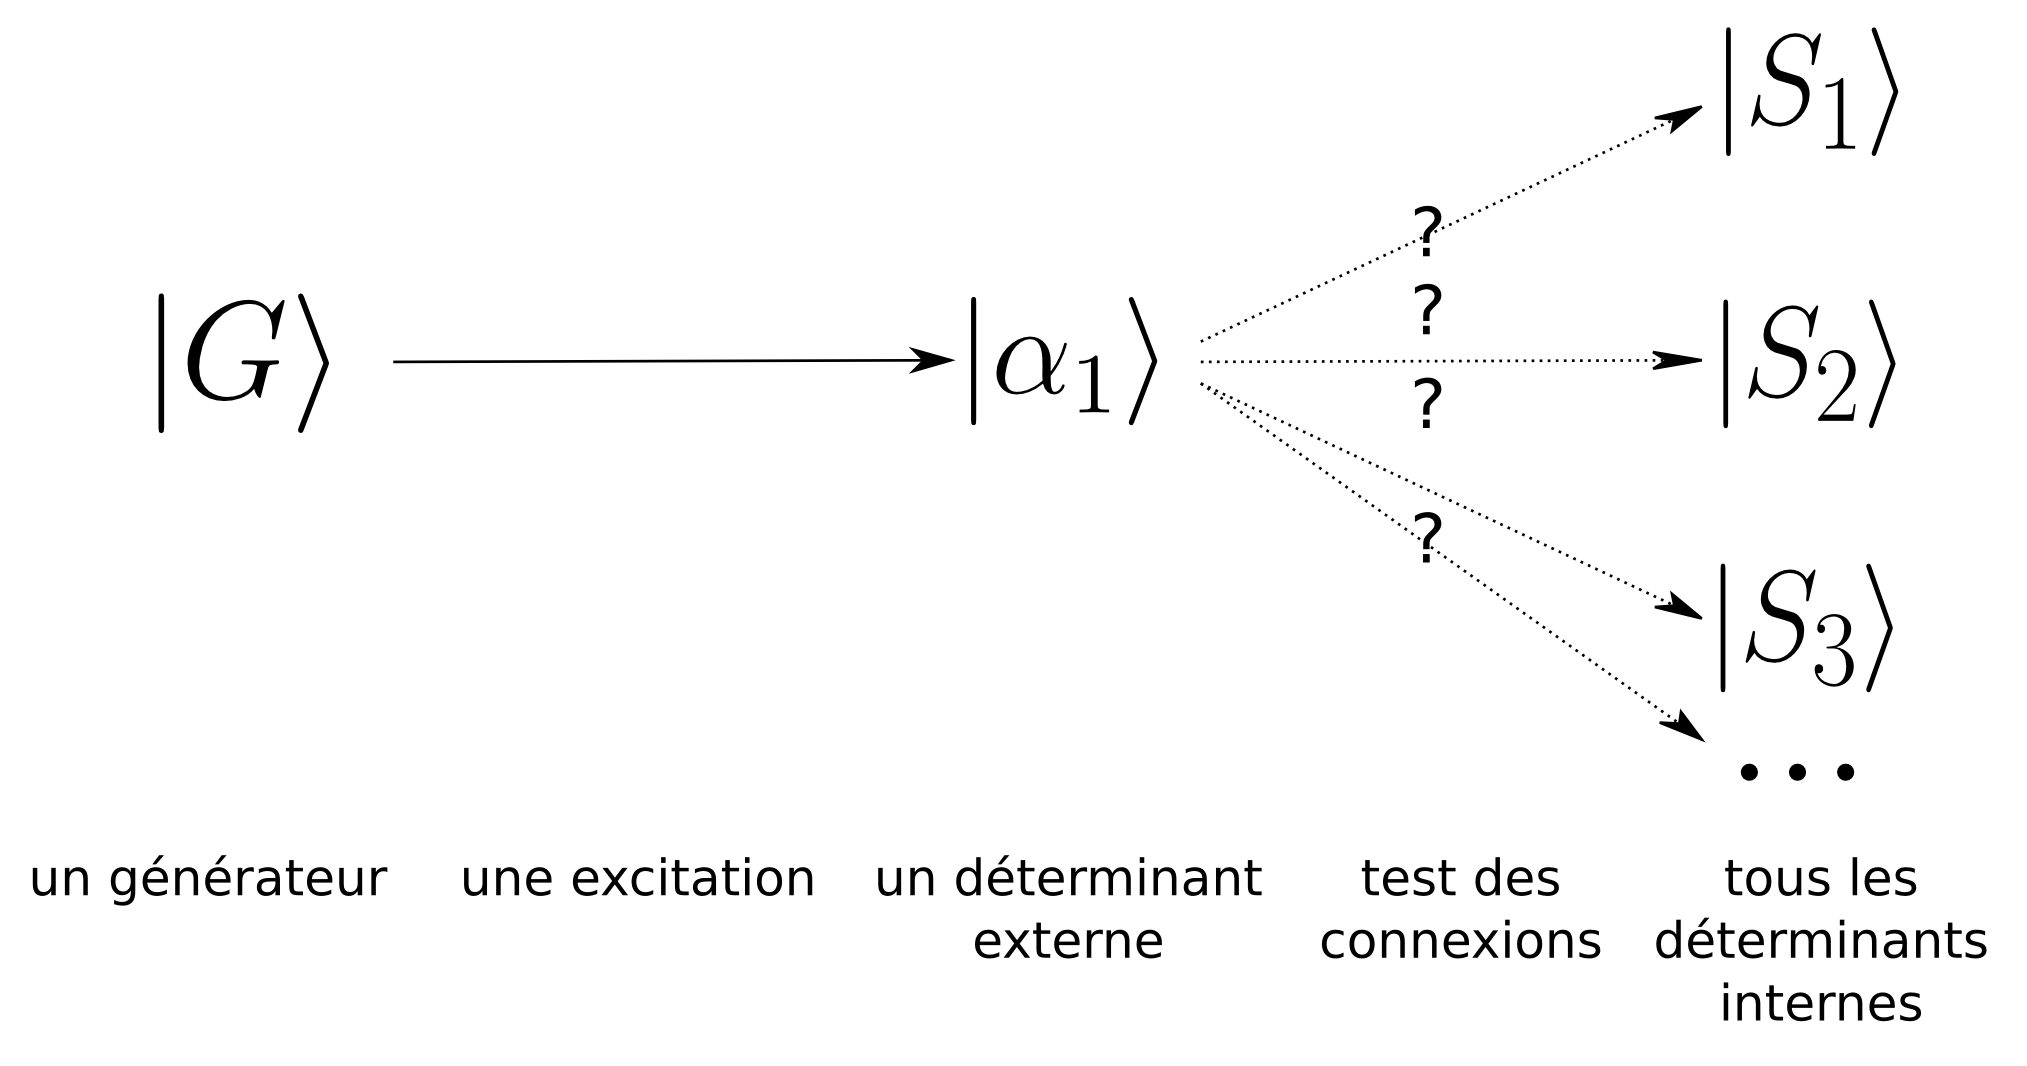
\includegraphics[width=0.6\columnwidth]{figures/cipsi/old_cipsi_fr}
        \end{center}
        \caption{Ancienne implémentation simple du CIPSI (représentation incomplète).}
        \label{fig:old_cipsi_fr}
\end{figure}
\begin{figure}[h!]
        \begin{center}
                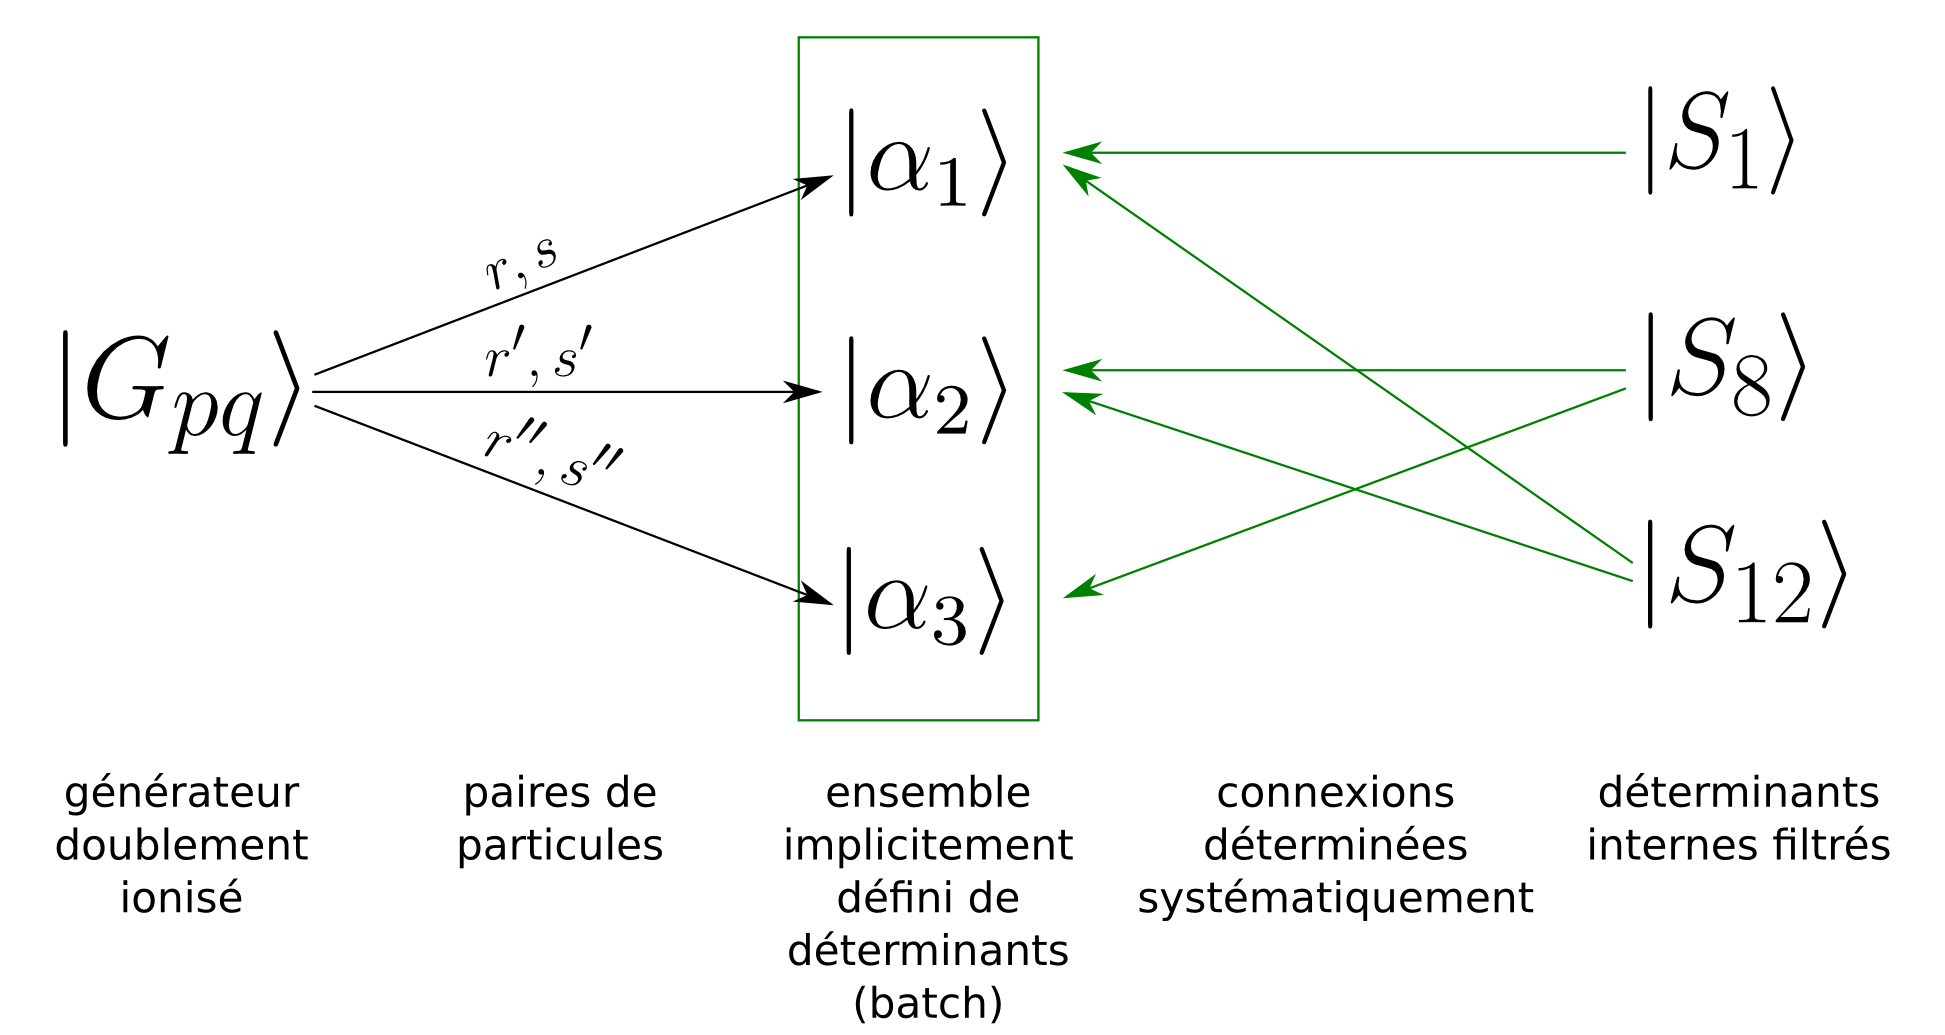
\includegraphics[width=0.6\columnwidth]{figures/cipsi/new_cipsi_fr}
        \end{center}
        \caption{Implémentation actuelle du CIPSI (représentation incomplète).}
        \label{fig:new_cipsi_fr}
\end{figure}
\section{Calcul de la contribution perturbative au second ordre}
La contribution perturbative au second ordre, qui donne accès à une valeur approximative de l'énergie Full-CI, est essentiellement la somme des contributions individuelles calculées au cours de l’algorithme CIPSI. Cependant son calcul est bien plus coûteux que celui du CIPSI, car moins d'approximations sont possibles. On peut également noter que la valeur exacte de $\EPT$ ne présente que peu d’intérêt, dans la mesure où elle ne sert que comme approximation de l'énergie Full-CI. De ce fait, un algorithme hybride stochastique/déterministe a été implémenté, donnant accès à $\EPT$ avec une précision suffisante pour une fraction du coût du calcul complet.
La contribution élémentaire n'est pas la contribution d'un seul déterminant externe, mais la somme pour 1 déterminant interne des contributions de tous les déterminants externes pouvant être générés à partir de lui mais d'aucun déterminant de coefficient supérieur en valeur absolue. La raison est d'abord technique, la somme des contributions de déterminants ``proches'' (en l’occurrence car tous connectés à un générateur particulier) peut être calculée efficacement. Les conséquences de ce regroupement sont:
\begin{itemize}
\item
Le nombre de contributions élémentaires est de $\Ndet$, et donc assez faible pour que chacune soit stockée en mémoire. Ainsi, contrairement au cas général dans un calcul Monte-Carlo, quand un élément est tiré, sa valeur peut être stockée et simplement ré-utilisée si cet élément est tiré à nouveau. On peut noter que la valeur exacte de $\EPT$ sera ainsi connue quand chaque élément aura été tiré, et donc pour un coût presque égale à celui du calcul exacte déterministe.
\item
Les valeurs absolues de ces contributions élémentaires décroissent rapidement avec le coefficient du générateur associé. 
\end{itemize}
Ce deuxième point guide la manière dont est conduit le calcul Monte-Carlo.

On tri les déterminants internes par coefficients absolus décroissants, par conséquent la majeure partie de la contribution est contenue dans le ``début'' de la fonction d'onde ainsi trié. Dans un premier temps on partage les déterminants en un intervalle déterministe $\mathcal{D}_D$ et un intervalle stochastique $\mathcal{D}_S$.

La partie déterministe, qui regroupe les contributions les plus importantes, est calculée entièrement. De ce fait la barre d'erreur ne porte que sur les plus petites contributions, ce qui permet de la réduire considérablement. La partie stochastique est séparée en intervalles appelés "dents" et notés $\mathcal{T}_1$, $\mathcal{T}_2$ ...   chacune contenant des contributions globalement plus faibles que celles de la dent précédente. Les valeurs qui serviront d'échantillon au sens statistique du terme, que l'on appel des \emph{peignes}, seront des sommes d'un déterminant tiré dans chaque dent ; en bref, la somme de ``un grand, un moyen et un petit'' aura en toute logique une variance plus faible que la somme de ``trois au hasard''. Lorsque toutes les contributions d'une dent ont été calculées, cette dent est déplacée dans la partie déterministe $\mathcal{D}_D$, ce qui permet de réduire encore la fraction des contributions sur laquelle porte la barre d'erreur. 

La figure ci-dessous résume ce procédé.
Chaque case correspond à un déterminant générateur, et sa largeur à la probabilité que ce déterminant soit tiré. La dent $\mathcal{T}_0$ est spéciale et fait toujours partie de $\mathcal{D}_D$, par conséquent aucun tirage n'est fait dedans. On a ici tiré deux peignes $a$ et $b$, dont les valeurs sont la somme des contributions des générateurs désignés par les flèches $a_1$, $a_2$, $a_3$ et $b_1$, $b_2$, $b_3$ respectivement.

Comme toutes les contributions de $\mathcal{T}_1$ ont été calculées, elles sont déplacées dans $\mathcal{D}_D$, et les générateurs 2 et 3 ne sont plus utilisés dans l'estimation stochastique, qui se fait uniquement avec les générateurs 6, 10 et 11.
 %\begin{figure}[h!]
        \begin{center}
                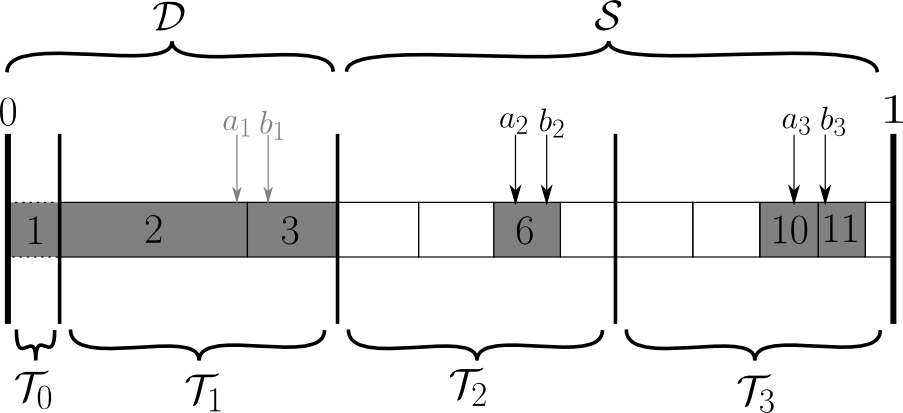
\includegraphics[width=0.75\columnwidth]{figures/pt2/toothindet}
        \end{center}
%               \caption{Illustrative example of drawing $n=2$ combs $a$ and $b$. Contributions that have been computed are greyed. $\mathcal{T}_1$ has been fully computed and is thus moved to $\mathcal{D}_D$. The first non-deterministic/not fully-computed tooth is $\mathcal{T}_{t=2}$.
%               $ E_D = e_1 + e_2 + e_3 $, 
%               $B_t(a) = W_T \Big ( \frac{e_6}{w_6} + \frac{e_{10}}{w_{10}} \Big ) \;;B_t(b) = W_T \Big ( \frac{e_6}{w_6} + \frac{e_{11}}{w_{11}} \Big )$, 
%               $E_S = \frac{B_t(a)+B_t(b)}{n}$}
%               \label{fig:toothindet_fr}
%\end{figure}
\section{Habillage stochastique de matrice}
Le calcul d'un habillage de matrice repose sur le même principe que le calcul de $\EPT$ ; la valeur recherchée est une somme dont chaque élément est associé à un déterminant externe. 

De la même manière que pour le calcul de $\EPT$, nous allons ici regrouper les contributions en $\Ndet$ ensembles chacun associé à un déterminant interne, ce qui nous donne $\Ndet$ contributions élémentaires.
Le chapitre ``Stochastic matrix dressing'' porte essentiellement sur la manière dont l'estimation est calculée à partir des contributions élémentaires ; le calcul de ces contributions élémentaires elles-mêmes, dans un cadre général, est développé dans le chapitre suivant, ``Application of stochastic matrix dressing to MR-CCSD''.

Un changement majeur est que ces contributions élémentaires, qui sont des scalaires dans le cas du calcul de $\EPT$, deviennent des vecteurs de taille $\Ndet$ dans le cas de l'habillage de matrice. Cela soulève une difficulté supplémentaire: il est possible de stocker $\Ndet$ scalaires, pas $\Ndet$ vecteurs de taille $\Ndet$. Comment alors éviter de ré-calculer une contribution si elle est tirée de multiples fois?

Cela a pu être réalisé par l’introduction de ``checkpoints'' pré-déterminés (d'une à quelques dizaines), en dehors desquels un résultat ne peut pas être obtenu. L'idée est que dans un schéma Monte-Carlo, même ``exotique'' comme notre schéma hybride déterministe/stochastique, le résultat estimé est une combinaison linéaire des échantillons. Avec $\deltabold^m$ l’estimation à un moment $m$ du calcul Monte-Carlo et $\deltabold_I$ la contribution élémentaire liée au déterminant interne d'indice $I$:
\begin{equation}
\deltabold^m = \sum_{I=1}^{\Ndet} \mu^m_{I} \deltabold_I
\end{equation}

On peut pré-calculer les coefficients $\mu_I^m$ de cette combinaison linéaire sans avoir accès à aucune contribution élémentaire. $\deltabold^m$ peut être initialisé au vecteur nul, puis construit incrémentalement au fur et à mesure que les contributions élémentaires sont calculées. Lorsque la contribution $\deltabold_I$ est calculée, le checkpoint $m$ et tous les autres sont mis à jour:
\begin{equation}
\deltabold^m \gets \deltabold^m + \mu^m_{I} \deltabold_I
\end{equation}
De cette manière la valeur $\deltabold_I$ n'a pas besoin d'être stockée.
 
\section{Application de l'habillage stochastique de matrice au MR-CCSD}

L'habillage de matrice, de manière générale, permet de raffiner la fonction d'onde variationnelle sous l'effet d'un espace externe. Cet espace externe est défini par une fonction $Z(\alpha,\ldots)$, prenant en paramètre au minimum un déterminant externe, et retournant le coefficient à lui associer. Afin de rendre simple l’implémentation de n'importe quel espace externe, un framework a été crée, dans lequel il suffit de définir cette fonction ; l'espace externe correspondant est estimé stochastiquement selon la méthode développée au chapitre précédent, et la fonction d'onde variationnelle est modifiée sous son effet.
Dans le cas de la méthode shifted-\Bk, dont il a été question dans le chapitre précédent, les coefficients externes sont estimés en perturbation. Dans ce chapitre, il s'agit des coefficients impliqués par la méthode MR-CCSD, qui avait précédemment été implémentée dans le cadre d'une publication.
 
De manière générale, la détermination d'un coefficient externe fait intervenir ses connexions avec l'espace variationnel. Pour des raisons de performance et de simplicité, il est vital que les déterminants internes auxquels se connecte le déterminant externe considéré, soient déterminés en amont de l'appel à la fonction $Z$ - le contraire contraindrait à ré-explorer la fonction d'onde entière pour chaque déterminant externe.

Nous avons pu réutiliser la ``machinerie'' du calcul CIPSI. En effet, dans ce dernier, chaque déterminant externe est mis en rapport avec tous les déterminants internes auxquels il se connecte, chaque connexion étant un apport à sa contribution perturbative. Dans le cas présent, quand une connexion sera mise en évidence, plutôt que d'incrémenter la contribution perturbative associée du déterminant externe impliqué, on ajoutera le déterminant interne à une liste associée au déterminant externe. A terme cette liste contiendra donc tous les déterminants internes connectés (voir figure \ref{fig:buildlists_fr}).
\clearpage

\begin{figure}[h!]
        \begin{center}
                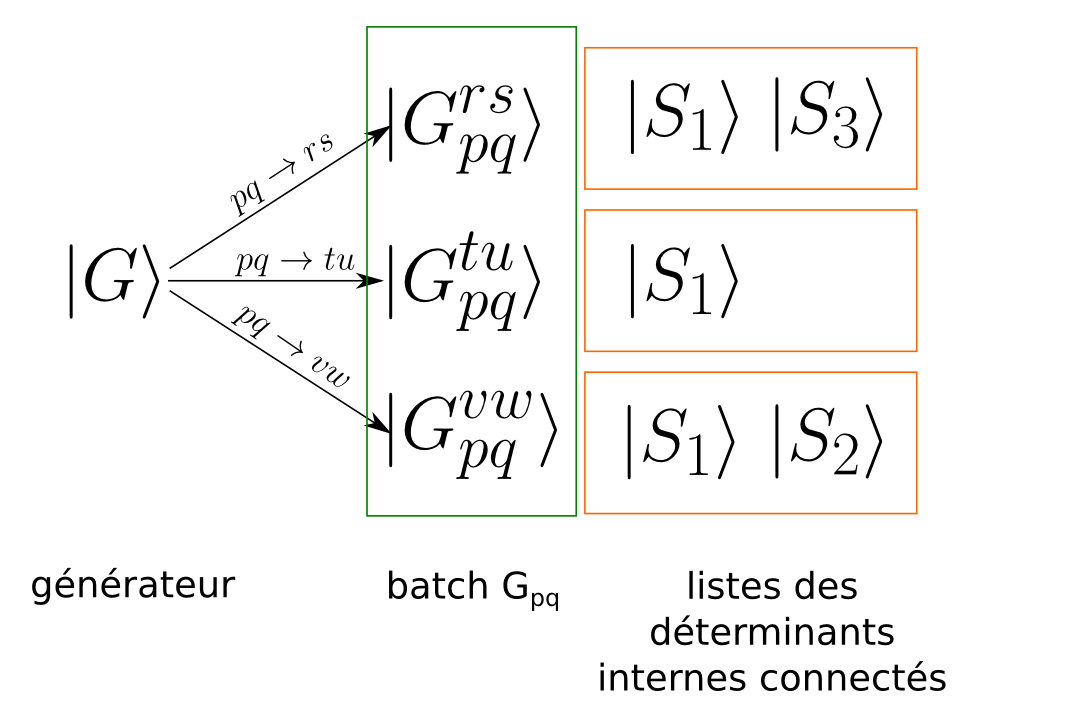
\includegraphics[width=0.7\columnwidth]{figures/matrix_dressing/buildlists_fr}
                \caption{Construction des listes de déterminants internes connectés pour tous les $\kalpha$ d'un batch $G_{pq}$.}
                \label{fig:buildlists_fr}
        \end{center}
\end{figure}
Dans le cas particulier du MR-CCSD, le calcul de ces coefficients se fait en mettant en évidence, pour chaque déterminant externe, des structures en ``losange''.
        \begin{center}
                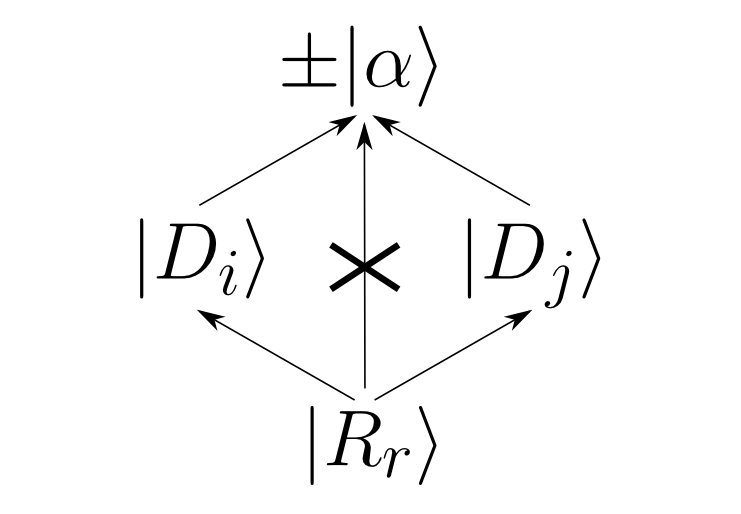
\includegraphics[width=0.3\columnwidth]{figures/matrix_dressing/diamond}
                %\caption{Build lists of connected selectors for unique $\kalpha$ in batch $G_{pq}$}
                %\label{fig:buildlists}
        \end{center}
        
Avec $\kalpha$ le déterminant externe considéré, $\ket {R_r}$ un déterminant de la référence, $\ket {D_I}$ et $\ket {D_J}$ deux déterminants internes. Les flèches parallèles indiquent une connexion par la même excitation. La flèche verticale indique une absence de connexion (degré d'excitation supérieur ou égale à 3).
On remarque que dans ce cas particulier, un losange peut être mis en évidence très simplement à l'aide de la fonction \texttt{IEOR} présentée précédemment, le critère étant:
\begin{equation}
\alpha \oplus D_I \oplus D_J \oplus R_r = 0
\end{equation}
Avec $\alpha$, $D_I$ ,$D_J$ et $R_r$ les $\uparrow \downarrow$-bitstrings définissants les déterminants correspondants, et $A \oplus B = \IEOR A B$. 
\clearpage

\section{Mesures de performance}
L'efficacité des implémentations est évaluée sur une cyanine, \\
\begin{center}
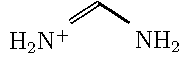
\includegraphics[]{figures/perf/Cyanine} \\
\end{center}
%[(NH$_2$)(CH)(NH$_2$)]$^+$
dans l'état fondamental et le premier état excité, en base aug-cc-pVDZ avec les orbitales $1s$ des atomes C et N gelées.

La géometrie est celle de l'état fondamental, optimisée au niveau PBE0/cc-pVQZ. L'état fondamental est de type couche fermée, bien décrit en mono-référence. L'état excité est simplement excité, et requiert deux déterminants dans la réference ($1/\sqrt{2} (a\bar{b} + b\bar{a})$).

L'espace Full-CI pour ce système est un CAS(18,111). L'énergie d'excitation de référence, obtenue au niveau CC3/ANO-L-VQZP, est de 7.18~eV.\cite{Send_2011}

Les calculs ont été effectués sur le supercalculateur Olympe (CALMIP), chaque nœud est un dual-socket Intel(R) Xeon(R) Gold 6140 CPU @ 2.30GHz avec 192Gio de RAM et 36 cœurs physiques.
Dans la figure ~\ref{fig:energy_pt2_fr}, on trace la convergence des énergies de l'état fondamental et de l'état excité en fonction du nombre de déterminants, avec et sans la contribution perturbative au second ordre $\EPT$.
On observe que, bien que $\EPT$ soit relativement grand ($\sim 0.02$~au), l'énergie d'excitation obtenue avec ou sans la correction perturbative est de $7.20$~eV, ce qui est compatible avec l'énergie de référence obtenue dans une base plus grande.
\begin{figure}[h!]
        \begin{center}
                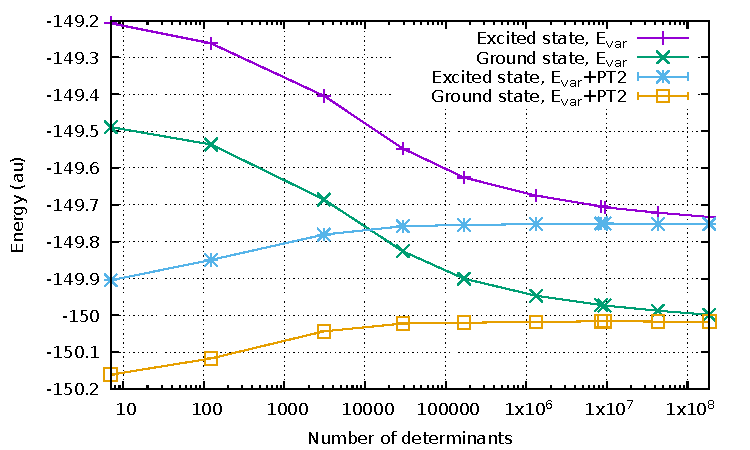
\includegraphics[width=0.75\columnwidth]{figures/perf/cn3_energy}
                \caption{               
                Convergence de l'énergie de l'état fondamental et de l'état excité en fonction du nombre de déterminants dans l'espace variationnel.}
                \label{fig:energy_pt2_fr}
        \end{center}
\end{figure}
\subsection{Diagonalisation de Davidson}
Nous mesurons le temps nécessaire à 1 itération de Davidson en fonction du nombre de déterminants dans la fonction d'onde variationnelle (figure \ref{fig:speedup_davidson_ndet_fr}).

Le scaling obtenu correspond à ce qui est attendu, à savoir  $\order{\Ndet^{3/2}}$.

Ensuite, en utilisant les deux plus grandes fonctions d'onde, nous mesurons le temps mural nécessaire au calcul en fonction du nombre de nœuds (figure \ref{fig:speedup_davidson_fr}).

Dans la mesure où la communication croît en $\order{\Ndet}$ alors que le calcul croît en $\order{\Ndet^{3/2}}$, l'efficacité parallèle augmente avec $\Ndet$.

Pour 50 nœuds avec la fonction d'onde à $42~959~496$ déterminants, l'efficacité parallèle est de 76\%

\begin{figure}[h!]
    \begin{center}
      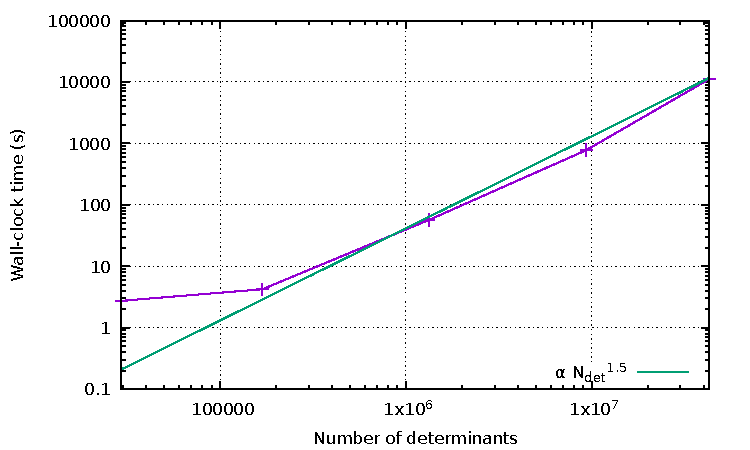
\includegraphics[width=0.80\columnwidth]{figures/perf/scaling_davidson_ndet}
      \caption{Temps mural d'une itération de Davidson en fonction du nombre de détermiants dans la fonction d'onde.}
      \label{fig:speedup_davidson_ndet_fr}
    \end{center}
\end{figure}
\begin{figure}[h!]
    \begin{center}
      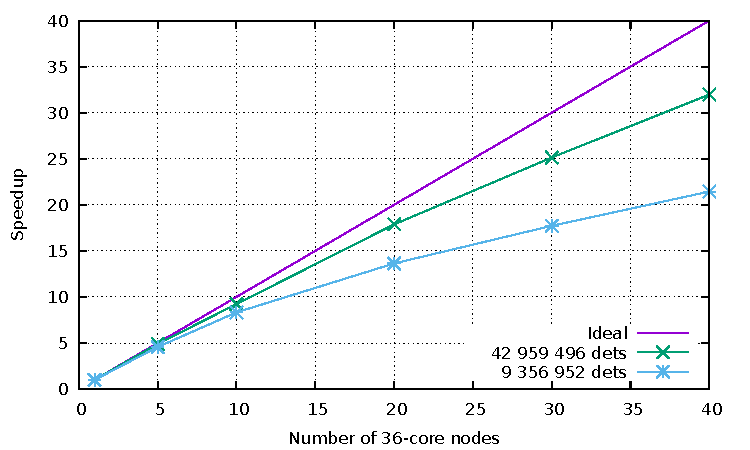
\includegraphics[width=0.80\columnwidth]{figures/perf/scaling_davidson}
      \caption{Accélération pour une itération de Davidson en fonction du nombre de noeuds à 36 cœurs.}
      \label{fig:speedup_davidson_fr}
    \end{center}
\end{figure}
\subsection{CIPSI}
Nous mesurons le temps nécessaire à une étape de sélection par CIPSI, en fonction du nombre de déterminants (figure \ref{fig:scaling_sel_ndet_fr}), puis du nombre de cœurs (figure \ref{fig:scaling_sel_node_fr}) avec la plus grande fonction d'onde ($9~356~952$ déterminants).
L'accélération en fonction du nombre de déterminant est presque idéale ; toutefois, cela est dû à une approximation (le seuil $n_g$, non discuté dans ce résumé), qui fait que le nombre de déterminants générateurs tend à devenir constant.
L'accélération en fonction du nombre de nœuds est également presque idéale, avec 95\% d'efficacité parallèle pour 50 nœuds. Cela est en partie dû à la fragmentation qui permet des tâches équilibrées.
\begin{figure}[h!]
    \begin{center}
      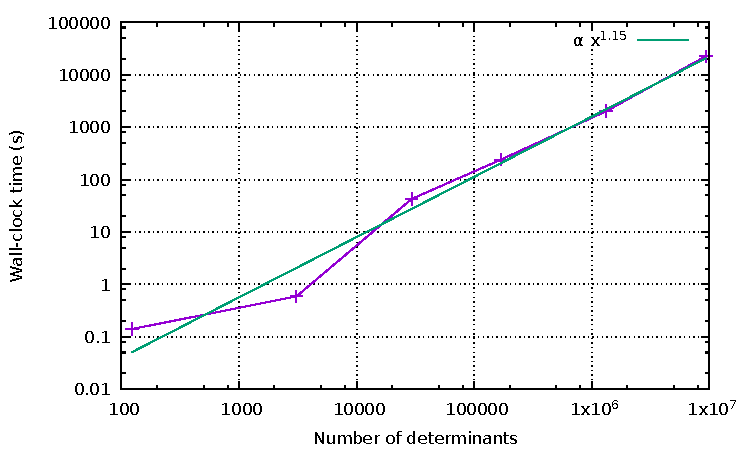
\includegraphics[width=0.8\columnwidth]{figures/perf/scaling_sel_det}
      \caption{Temps mural de la sélection CIPSI en fonction du nombre de déterminants dans la fonction d'onde.}
      \label{fig:scaling_sel_ndet_fr}
    \end{center}
\end{figure}
\begin{figure}[h!]
    \begin{center}
      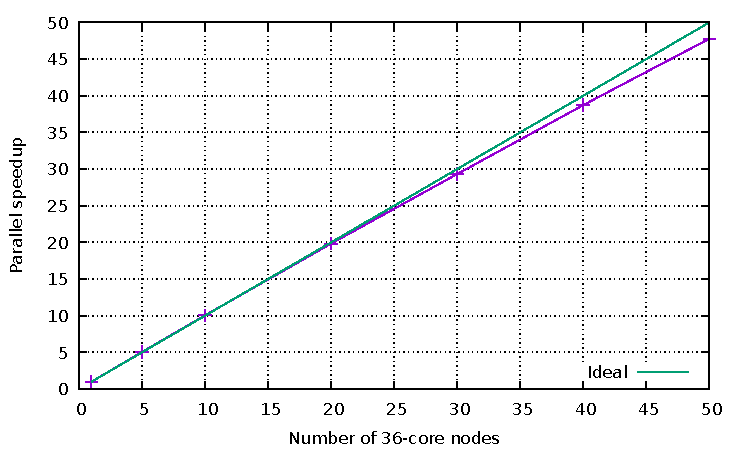
\includegraphics[width=0.8\columnwidth]{figures/perf/scaling_sel_node}
      \caption{Accélération parallèle pour la sélection CIPSI. La référence est un unique nœuds à 36 cœurs.}
      \label{fig:scaling_sel_node_fr}
    \end{center}
\end{figure}
\subsection{Calcul de $\EPT$}

L’algorithme du calcul de $\EPT$ est très similaire à celui du CIPSI. On s'attend donc à un comportement similaire.

Le critère d'arrêt est une erreur relative de 1/1000. Puisque $\EPT$ diminu avec $\Ndet$, l'erreur acceptable diminue également avec $\Ndet$. Cependant, le coût du calcul stochastique par rapport au calcul complet reste relativement constant, autour de 5\%.

Le scaling obtenu en fonction de $\Ndet$ (figure \ref{fig:scaling_det_pt2_fr}) est presque linéaire, $\order{\Ndet^{1.15}}$, pour les plus grandes fonctions. Cela peut se comprendre, dans la mesure où pour un relativement petit nombre de déterminants, le nombre de déterminants externes produit est proportionnel à $\Ndet$, chacun potentiellement connecté à $\Ndet$ déterminants internes, pour un scaling attendu de l'ordre de $\Ndet^2$. Toutefois, à mesure que la fonction variationnelle tend vers la fonction Full-CI, le nombre de déterminants internes auxquels un déterminant externe est connecté, est limité par le nombre de doubles excitations possibles, ce qui fait disparaître la seconde dépendance à $\Ndet$.

Le scaling obtenu en fonction du nombre de nœuds (figure \ref{fig:scaling_node_pt2_fr}) est un peu moins satisfaisant que celui obtenu pour le CIPSI. L'efficacité parallèle avec 50 nœuds (1800 cœurs) est de 80\%, contre 95\% pour le CIPSI. On peut trouver deux raisons à cela:
\begin{itemize}
\item
Le pré-calcul des peignes sur le processus maître délaye le début de la partie parallèle.
\item
Contrairement au CIPSI, le calcul est ici interrompu de manière imprévisible, lors que la barre d'erreur atteint le seuil requis. Par conséquent un certain nombre de tâches ``superflues'' peuvent être lancées, ce nombre étant d'autant plus grand que le nombre de cœurs est important ; dans la limite où $\Ndet$ est égal au nombre de cœurs, c'est de fait toujours le calcul complet qui sera réalisé, alors que dans le mode mono-cœur aucune tâche superflue ne sera calculée.
\end{itemize}

Les tâches qualifiées de superflues pouvant néanmoins être utilisées pour réduire la barre d'erreur, ce calcul d'accélération n'est pas tout à fait pertinent car la barre d'erreur finale sera plus faible quand le nombre de nœuds est plus grand.


\begin{figure}[h!]
        \begin{center}
                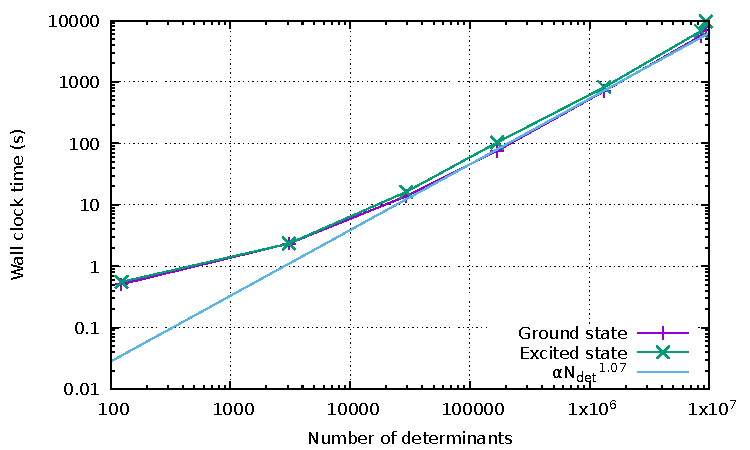
\includegraphics[width=0.8\columnwidth]{figures/perf/scaling_pt2_det}
                \caption{Temps mural requis pour calculer la contribution perturbative $\EPT$ pour l'état fondamental et l'état excité, en fonction du nombre de déterminants dans la fonction d'onde.            }
                \label{fig:scaling_det_pt2_fr}
        \end{center}
\end{figure}
\begin{figure}[hbt!]
        \begin{center}
                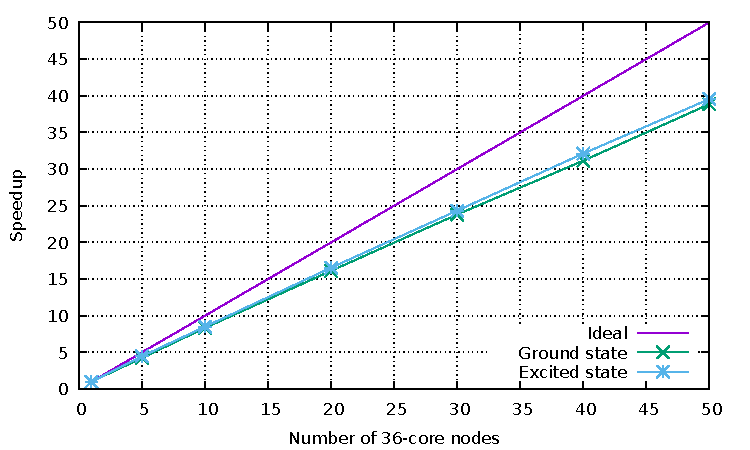
\includegraphics[width=0.8\columnwidth]{figures/perf/scaling_pt2_node}
                \caption{Accélération parallèle pour le calcul de la contribution perturbative $\EPT$ pour l'état fondamental avec la plus grande fonction d'onde. Chaque nœud contient 36 cœurs physiques.               }
                \label{fig:scaling_node_pt2_fr}
        \end{center}
\end{figure}
%\clearpage
\subsection{Habillage de matrice}

L'algorithme d'habillage de matrice est similaire à celui du calcul de $\EPT$, on s'attend donc à un comportement similaire.

Le critère d’arrêt est une erreur relative de 1/1000 sur l'énergie d'habillage $\mel{\Psi}{\hat \Delta}{\Psi}$, avec $\hat \Delta$ la matrice d'habillage.

Le scaling en fonction du nombre de déterminants (figure \ref{fig:scaling_det_sbk_fr}) est de $\order{\Ndet^{1.15}}$, ce qui est légèrement supérieur à celui trouvé pour $\EPT$. 

Ce coût additionnel est lié à la gestion des résultats par checkpoint, qui élimine le goulot d'étranglement lié aux communications. 

L'accélération en fonction du nombre de nœuds (figure \ref{fig:scaling_node_sbk_fr}) a été mesurée avec la fonction d'onde à $9~356~952$ déterminants.

\begin{figure}[h!]
        \begin{center}
                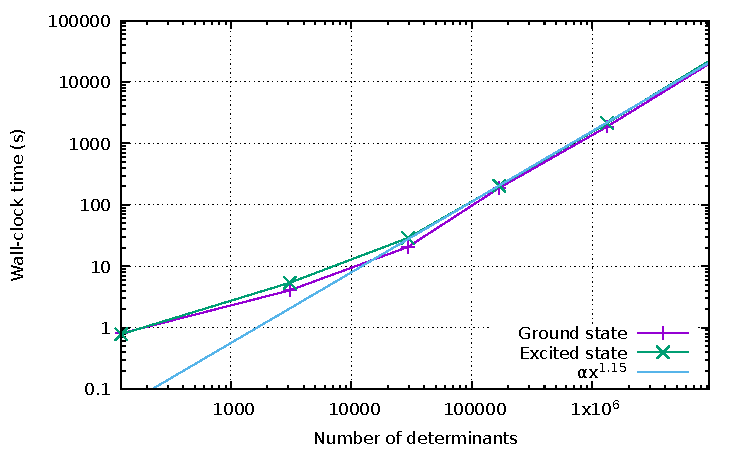
\includegraphics[width=0.8\columnwidth]{figures/perf/scaling_sbk_det}
                \caption{Temps mural requis pour calculer l'habillage Shifted-$B_k$ pour l'état fondamental et l'état excité, en fonction du nombre de déterminants dans la fonction d'onde.}
                \label{fig:scaling_det_sbk_fr}
        \end{center}
\end{figure}
\begin{figure}[hbt!]
        \begin{center}
                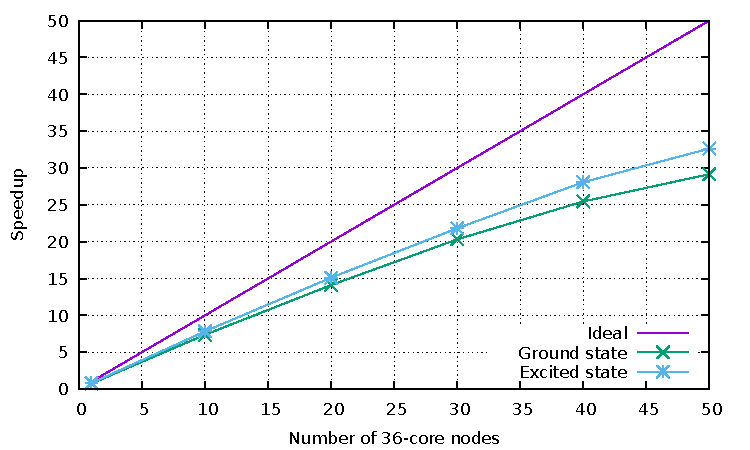
\includegraphics[width=0.8\columnwidth]{figures/perf/scaling_sbk_node}
                \caption{Accélération parallèle pour le calcul de la matrice d'habillage de l'état fondamental avec la plus grande fonction d'onde. Chaque noeud contient 36 cœurs physiques.}
                \label{fig:scaling_node_sbk_fr}
        \end{center}
\end{figure}

%\clearpage

\section{Conclusion}

Des améliorations aussi bien dans le mode séquentiel que parallèle ont été apportées au \QP. Il est actuellement possible de réaliser des calculs sur $\sim 2000$ cœurs avec des centaines de millions de déterminants dans l'espace variationnel, ce qui pourra conduire à la réalisation d'autres d'applications difficiles.

La diagonalisation de Davidson, au centre des méthodes variationnelles, souffre de l’impossibilité de stocker la matrice hamiltonienne, ce qui nous contraint à recalculer les éléments de matrice \emph{on the fly} à chaque itération. Malgré une méthode très efficace pour calculer les éléments de matrice,\cite{Scemama_2013} et en particulier pour identifier un élément nul, l'implémentation initiale explorait chacun des $\sim \Ndet^2$ éléments de matrice.

À présent, les déterminants sont séparés en plusieurs ensembles disjoints et souvent identifiables comme entièrement déconnectés les uns des autres ; de ce fait, la vaste majorité des éléments de matrice n'ont plus à être explicitement considérés, et le scaling est ramené à $\order{\Ndet^{3/2}}$. Une variante de scaling linéaire est possible, mais n'a pas été implémentée du fait d'une empreinte mémoire trop importante. Cependant, l'implémentation pourrait être raffinée afin d'utiliser conjointement les deux méthodes.

Bien que la parallélisation de l'algorithme proposé soit difficile, l'implémentation distribuée qui en a été réalisée offre une accélération satisfaisante, de l'ordre de $35\times$ pour $50$ nœuds ($1~800$ cœurs). 

L'algorithme de sélection CIPSI a été considérablement amélioré, ce qui a rendu possible des applications jusque là infaisables.\cite{Scemama_2018,1806.05115}

Les différentes optimisations réalisées portent à la fois sur la mise en évidence des connexions entre les espaces interne et externe (approche par batch de déterminants, filtrage), et le coût de calcul des éléments de matrice correspondants (phase mask, détermination implicite des excitations).
L'implémentation distribuée offre une accélération presque idéale avec 50 nœuds.

D'un point de vue méthodologique, le CIPSI est toutefois d'une précision et donc d'un coût qui ne se justifie pas dans toutes les situations ; de meilleurs performances, sans perte de précision, pourraient être obtenues en combinant le CIPSI avec un algorithme de sélection moins précis mais très peu coûteux, le \emph{Heat-Bath Configuration Interaction (HCI)}. \cite{Holmes_2016, Sharma_2017}

Le calcul de la contribution perturbative au second ordre $\EPT$, a également fait l'objet d'améliorations importantes. Bien qu'étant calculé par le même algorithme que CIPSI, obtenir $\EPT$ était plus coûteux car n'autorisant pas autant d'approximations. Dans la mesure où $\EPT$ est une somme d'une multitude de termes, une approche Monte-Carlo est pertinente, d'autant plus que $\EPT$ sert essentiellement à fournir une approximation de l'énergie Full-CI. Par conséquent, sa valeur exacte n'a que peu d’intérêt, l'important étant que la précision de son estimation soit supérieur à la précision typique avec laquelle $E_{\text{var}} + \EPT$ approxime l'énergie Full-CI.

L'approche Monte-Carlo proposée, originale par son caractère hybride stochastique/déterministe, a été développée avec l'aide du groupe de Michel Caffarel, et permet d'obtenir $\EPT$ avec une précision satisfaisante pour quelques pourcents du coût du calcul exacte.

Toutefois, cette approche stochastique n'est utilisée que pour le calcul de $\EPT$ et pas pour la sélection. Une sélection stochastique aurait l'avantage qu'à chaque itération, n'importe quel déterminant externe pourrait potentiellement être généré. Ce n'est pas le cas avec l'approche actuelle, en raison du seuil $n_g$, les déterminants de faibles coefficients ne sont jamais utilisés comme générateurs, ce qui est la cause d'une légère erreur de size-consistance.

Afin de tirer le meilleur parti des données auxquelles nous pouvions déjà accéder, nous avons par la suite implémenté la méthode shifted-\Bk, qui permet de raffiner la fonction d'onde en fonction des contributions énergétiques individuelles des déterminants externes. Cette méthode nécessite le calcul d'une matrice d'habillage, estimée stochastiquement de la même manière que $\EPT$. Toutefois, de part le fait que l'estimation porte sur un vecteur et non plus sur un scalaire, des difficultés supplémentaires ont dû être surmontées. Cela a pu être fait au prix d'un compromis relativement modeste, consistant à pré-définir, au début du calcul, un certain nombre (de l'ordre d'une à quelques dizaines) de ``checkpoints'' au niveau desquels un résultat est obtenu ; entre deux checkpoints, aucun résultat n'est disponible.

Cet habillage stochastique de matrice a ensuite pu être généralisé dans un framework permettant de raffiner la fonction d'onde sous l'effet de n'importe quel espace externe (défini par les coefficients des déterminants externes). Une implémentation de la méthode \emph {Multi-Reference Coupled Cluster Single and Double (MR-CCSD)} a ainsi pu être réalisée simplement,\cite{Garniron_2017} et a permis d'explorer certaines possibilités de l'approche determinant-driven. 

A l'heure actuelle ce framework est commode mais offre peu de possibilités. Certaines pistes sont explorées afin de le rendre plus flexible.

Durant les différentes étapes de l'évolution du \QP, de plus en plus d'applications ont été rendues possibles.\cite{Loos_2018,Garniron_2018,Giner_2017,Garniron_2017,Garniron_2017b,Scemama_2018,1806.05115}

Cela a donné au \QP plus de visibilité, conduisant notamment à sa sélection en tant que benchmark dans le choix du nouveau supercalculateur du centre CALMIP. De plus, différents groupes se sont mis à l'utiliser pour des applications et le développement de nouvelles idées. Par exemple, le groupe de Claudia Filippi aux Pays-Bas utilise maintenant des fonctions d'onde CIPSI dans le cadre de calculs Monte-Carlo quantique,\cite{Dash_2018} et le groupe d'Argonne implémente actuellement des orbitales complexes afin d'adapter le \QP à la chimie du solide.\cite{Benali_2018}
\end{document}